\documentclass[12pt]{article}
\usepackage{graphicx}
\begin{document}
\title{Document Tender}

\begin{titlepage}
\begin{huge}
\begin{center}
Project Tender

Project: SMART Sensing AI
\\
\begin{LARGE}
Client: Willburg Outdoor
\end{LARGE}

Team: Dragon Brain
\\
\begin{small}
Department of Computer Science, University of Pretoria
\\
\begin{itemize}
\item Matheu Botha u14284104
\item Renton McIntyre u14312710
\item Emilio Singh u14006512
\item Gerard van Wyk u14101263
\end{itemize}


Date: 2016/05/02

\end{small}


\includegraphics[scale=0.2]{test}
\end{center}

\end{huge}


\end{titlepage}

\pagebreak

\section{The Team}
\subsection{Matheu Botha}
\includegraphics[scale=0.02]{Matheu}
\paragraph{Interests}
My main interests lie in Artificial Intelligence. This is applicable to the project as pattern recognition is largely considered one of the more difficult areas in computer science and some of the most progressive solutions have come from artificial intelligence algothrithms.

\paragraph{Technical Skills}
	I am proficient in the following programming languages:
	\begin{itemize}
		\item C++
		\item C#
		\item Java
		\item Javascript
		\item Python
		\item PHP
	\end{itemize}

\paragraph{Relevant Past Experience}
	In the past I have done projects with Monkey and River developing the SALGA Municipal Barometer. I have also worked with Merlynn Intelligent Technologies developing the UP2TOM app. Both of these projects involved extensive Front End development which has given me experiance with regard to developing User Interfaces, which is relevant for the project. I have also been working as a part time technical assistant for the university of pretoria which has afforded me the opportunity to work with many enterprise level development technologies in a production environmet.

\paragraph{Non-technical Strengths}
	I enjoy working as part of a team on a large project. I am also very challenge driven. I enjoying taking on challenging projects and working hard with a group of like minded individuals to overcome those challenges.

\paragraph{Motivation for Project}
	I would like to work on this project because it is a very progressive field that still has the potential for a lot of innovative work to be done in it.

\subsection{Renton McIntyre}

\includegraphics[scale=0.25]{Renton}
\paragraph{Interests}
My relevant interests include the fields of Artificial Intelligence and general academic advancement and experimentation.
\paragraph{Technical Skills}
I have had prolonged exposure to Java and C++ (the latter of which I consider to be my primary language). I also have experience with various scripting languages, C and Assembly.

Otherwise, I have some mathematical prowess and, perhaps above all else, a proficiency in the ability to learn technical skills on short notice.
\paragraph{Relevant Past Experience}
I have very few past experience with such projects. However, I am willing to learn and believe I will be able to make a valuable contribution towards the project.

\paragraph{Non-technical Strengths}
I believe I have a strong capability to work with people and have previously shown my ability to maintain my connection with a team well, often from the perspective of serving as somewhat of an assistant to the person in charge, as I do not often take such a role myself, despite potentially having the capability. 
\newline I also believe I have a good ability to apply concepts to practicality.
\paragraph{Motivation for Project}
The suggested Smart Image project piques my interest with its strong involvement in the field of Artificial Intelligence and specifically neural networks, in which I have recently developed a larger interest. Additionally, I think the project's aim is very respectable and although the task of object identification is not a simple one, I believe the purpose for which the project is planned to be used has great moral benefits.

\subsection{Emilio Singh}
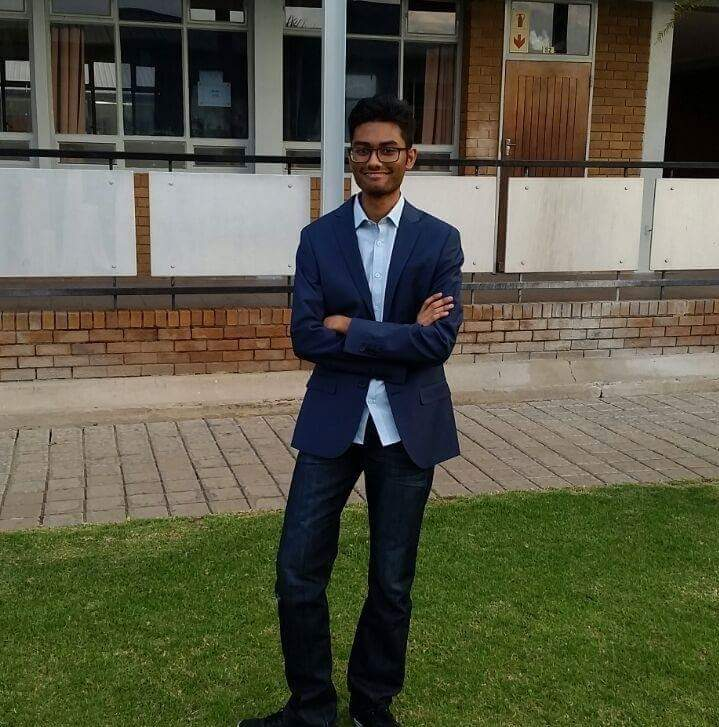
\includegraphics[scale=0.2]{Emilio}
\paragraph{Interests}
My relevant interests include the study of cryptography, video games and reading.
\paragraph{Technical Skills}
I can program using Java, C++, and a variety of scripting languages proficiently.
Furthermore, I have exposure, and somewhat fluency in Assembly.

My true strength would be in the field of mathematics and analysis however as I have shown high level competencies in various mathematical subjects while at university.
\paragraph{Relevant Past Experience}
Other than the 301 Mini Project, I have no worked on any major software system to this caliber but rest assured, I am very eager to learn and contribute towards the project.
\paragraph{Non-technical Strengths}
In terms of non-technical strengths, I would say that I have a capacity to serve in a leadership role. I have proven on numerous occasions that I can work with others and coordinate them towards a particular aim.

Furthermore, I feel that I have a level of skill with regards to communication with people from both technical and non-technical backgrounds which would typically aid in client-team communications.
\paragraph{Motivation for Project}
The Smart Image project appeals to me because I have only recently begun to explore the field of data classification and classification problems as a whole using neural networks. The idea of using image analysis or classification to help create a software system meant to help protect people is a noble one and I believe the project has merit because of this.

\subsection{Gerard van Wyk}
\includegraphics[scale=0.02]{a}
\paragraph{Interests}
I am highly interested in Artificial Intelligence, video games/virtual reality and reading about science(especially space, geology and natural selection).
\paragraph{Technical Skills}
My programming language proficiencies are in Java, C++, and to a lesser extent OpenGL and general web languages.
Aside from programming languages: I am good at mathematics, and have a moderate skill in image and video editing.
\paragraph{Relevant Past Experience}
I have not had previous experience with large software engineering projects other than the smaller COS 301 mini-project, however I am
eager to learn and dive into this new experience.
\paragraph{Non-technical Strengths}
I work well with other people, learn quickly, am driven by intellectual curiosity, and always seek to achieve an efficient solution.
\paragraph{Motivation for Project}
I have always been deeply interested in artificial intelligence, and this project is an opportunity to tackle a very hard AI problem: pattern recognition. It may seem trivial in concept but a simple "Human detector" is an exremely hard problem that even the likes of Google has not fully solved yet, I am however not deterred and would love to have the chance to try and build such a powerful and useful system.

\section{Project Execution}
\section{Project Execution}
\paragraph{Developmental Methodology}
We will be following an Agile development methodology. We hope to realise this development methodology by doing the following:
\begin{enumerate}
\item Communicating with our clients to ensure they are informed of project progress as well as to constantly refine and update our understanding of requirements in order to meet them.
\item Construct a frequent, working software delivery schedule so that incrementally working segments of the STORM project can be delivered to our clients.
\item Commit to the delivery of simplistic, maintainable and efficient software.
\item Accept that requirements for the project may change constantly throughout the project life-cycle and develop a modular system whose functioning can be easily adapted to suit this purpose.
\item We have a strong commitment to compartmentalisation of work and will adopt pair-programming and other team-oriented development practices as we are able to.
\end{enumerate}

\paragraph{Client-Team Communication Methods}
We will make use of the contact details provided to initiate contact so that we may establish what manner of personal, face-to-face communication we can arrange with the client to better understand the project's constraints, requirements and needs. Furthermore, we will use emails as and when necessary to request communications.

Finally, we have also created a Slack group to manage the project team for the duration of the project. The clients will be extended the offer to join the group to be more directly related to intra-team communications.
\paragraph{Initial Ideas in response to Technical Challenges}
\paragraph{Potential Technologies for use where not specified by client}
\paragraph{Deliverable to Client}
\end{document}
